%qepaper.tex
\documentclass[12pt,letterpaper]{article}
\usepackage{mathptmx}
\usepackage[margin=1in]{geometry}

\usepackage{tabularx, longtable, pdflscape, adjustbox}  % for 'tabularx' environment and 'X' column type
\usepackage{ragged2e}  % for '\RaggedRight' macro (allows hyphenation)
\newcolumntype{Y}{>{\RaggedRight\arraybackslash}X} 
\usepackage{booktabs}  % for \toprule, \midrule, and \bottomrule macros 

\usepackage{setspace}
\onehalfspacing
%\doublespacing
%\singlespacing

\usepackage{amssymb,latexsym}
\usepackage[round,sort]{natbib}
\usepackage{fancyhdr}
\usepackage{lastpage}
\usepackage{graphicx,multirow}
\graphicspath{ {qepaper/} }

% Bold Table and Figure captions
\usepackage{caption}
\captionsetup{figurename=FIGURE}
\captionsetup{tablename=TABLE}
\captionsetup[figure]{labelfont=bf}
\captionsetup[table]{labelfont=bf}

% Turns off all section numbering
\setcounter{secnumdepth}{0} 

\usepackage{titling}

  % Places all tables at end of document and creates AOM-style table-here placeholders
  \usepackage[nolists]{endfloat} % Places all figures and charts at end of manuscript and adds 'insert table x about here' lines.
  \renewcommand{\figureplace}{
    \begin{center}
    \begin{singlespace}
    ------------------------------------\\
    Insert \figurename \ \thepostfig\ about here.\\
    ------------------------------------
    \end{singlespace}
    \end{center}}
  \renewcommand{\tableplace}{%
    \begin{center}
    \begin{singlespace}
    ------------------------------------\\
    Insert \tablename \ \theposttbl\ about here.\\
    ------------------------------------
    \end{singlespace}
    \end{center}}

  \usepackage{titlesec}
   \titleformat{\title}
       {\filcenter\normalfont\bfseries\uppercase}{\thetitle}{1em}{}
  \titleformat{\section}
    {\filcenter\normalfont\bfseries\uppercase}{\thesection}{1em}{}
  \titleformat{\subsection}
    {\normalfont\bfseries}{\thesubsection}{1em}{}
  \titleformat{\subsubsection}[runin]
   {\normalfont\bfseries\slshape}{\thesubsubsection}{1em}{\hspace*{\parindent}}
       
\usepackage{tabu}
\usepackage{textcomp}
\usepackage{listings}
\usepackage{hyperref}
\usepackage{verbatim}
\usepackage{tabu}
\hypersetup{
    colorlinks=true,
    linkcolor=blue,
    filecolor=cyan,      
    urlcolor=cyan,
    citecolor=blue,
}

\usepackage{etoolbox}

\makeatletter

% Patch case where name and year are separated by aysep
\patchcmd{\NAT@citex}
  {\@citea\NAT@hyper@{%
     \NAT@nmfmt{\NAT@nm}%
     \hyper@natlinkbreak{\NAT@aysep\NAT@spacechar}{\@citeb\@extra@b@citeb}%
     \NAT@date}}
  {\@citea\NAT@nmfmt{\NAT@nm}%
   \NAT@aysep\NAT@spacechar\NAT@hyper@{\NAT@date}}{}{}

% Patch case where name and year are separated by opening bracket
\patchcmd{\NAT@citex}
  {\@citea\NAT@hyper@{%
     \NAT@nmfmt{\NAT@nm}%
     \hyper@natlinkbreak{\NAT@spacechar\NAT@@open\if*#1*\else#1\NAT@spacechar\fi}%
       {\@citeb\@extra@b@citeb}%
     \NAT@date}}
  {\@citea\NAT@nmfmt{\NAT@nm}%
   \NAT@spacechar\NAT@@open\if*#1*\else#1\NAT@spacechar\fi\NAT@hyper@{\NAT@date}}
  {}{}

\lstset{
basicstyle=\ttfamily,
columns=flexible,
breaklines=true
}
\newenvironment{hypothesis}{
  	\itshape
  	\leftskip=\parindent \rightskip=\parindent
  	\noindent\ignorespaces}

\fancypagestyle{plain}{
  \renewcommand{\headrulewidth}{0pt}
  \fancyhf{}
}	

\begin{document}
\setlength{\droptitle}{-5em}
\title{\textbf{\large Heterogeneity in Knowledge Flows of Regions: Impact on Invention Quality}}
\date{\vspace{-12ex}}

\maketitle
\thispagestyle{empty}
\renewcommand{\abstractname}{\normalsize ABSTRACT}
\begin{abstract}
\normalsize
\noindent Using patent citations as measures of knowledge flows, we explore if the different types of knowledge flows in a region affect the quality of inventions originating in that region. We leverage a database of worldwide urban centers  obtained from remote sensing data and find that  local knowledge flows  do not seem to impact the inventive quality of regions. However, knowledge flows within the firm across regions seem to have a positive effect on invention quality. 
\end{abstract}

\newpage
\pagestyle{fancy}
\fancyhf{}
\lhead{Heterogeneity in Knowledge Flows of Regions: Impact on Invention Quality}
\rhead{\thepage}

\textbf{Heterogeneity in Knowledge Flows of Regions: Impact on Invention Quality}

\vspace{3ex}


\noindent Empirical studies in the literature on economic geography have used patent citations to suggest that knowledge spillovers are geographically localized \citep*{Jaffe1993, Almeida1999, Alcacer2006a, Bottazzi2003, Branstetter2001, Maurseth2002, Sonn2008}, and that innovation is more spatially concentrated that production \citep{Feldman1994a}. On the other hand, patent citations have also been used in the international business literature to demonstrate that multi-national firms (MNCs) gain from the cross-border flow of knowledge and the globalization of R\&D \citep{Singh2007, Zhao2006, Singh2013}. This leads to the question of what indeed is the net effect of geography on innovation outcomes of firms and regions. Firms seek to improve innovation outcomes as a way of building a sustainable competitive advantage. Understanding how knowledge flows across firms and geographies affect innovation outcomes would be valuable to managers in their quest for superior performance. \par

In this study, we\footnote{This paper is the outcome of the joint work by my co-author and me. While the changes since the version submitted to a conference in February 2017 (sms2017.pdf, provided as supplementary material) are without consultation with my co-author, I have used the plural ``we'' throughout this paper to preserve continuity with the previous version and compatibility with future versions that are going to be jointly authored.} examine how the nature of knowledge spillovers or flows in a region affect the quality of the inventions generated in the region. Specifically, we look at knowledge flows spanning region boundaries and firm boundaries, and ask if and to what extent prior knowledge flows between and within regions and firms affects innovation quality of patents originating in a region. In this study we use citation data of patents applied for between 2001 and 2012 to empirically estimate the relationship between knowledge flows of a region and quality of inventions from that region. We are aware of no prior studies that have examined the effects of the geographical characteristics of knowledge flows on invention outcomes of regions. Our work therefore seeks to contribute to the innovation literatures in both economic geography and international business. \par 

It would seem appropriate to raise two measurement related issues here soon after we propose our research question. First, despite well known issues in the use of patents \citep{Griliches1990, Scherer1984} and in the use of patent citations to demonstrate localization of knowledge spillovers \citep*{Thompson2005, Arora2017a}, much work in understanding knowledge spillovers has continued to rely on patent citations. While our analysis in this paper is singularly dependent on data of United States patents, we are careful to not make strong assumptions about patent citations reflecting underlying knowledge flows. Wherever possible, we consider competing hypotheses built on opposing assumptions about what patent citations may capture. Second, innovations are clearly not the same as inventions. The measure of an innovation lies in its acceptance in the marketplace. An invention may therefore only represent an early event in the innovation process. While we recognize that managers and policy makers are interested in innovation outcomes, we continue to be limited by data availability that allows us to only make claims about invention quality. Despite those caveats, pursuing the questions posed above can provide not just interesting trade-offs to explore, but indeed create opportunities for a larger research agenda on actionable strategies for firms seeking to improve their innovation outcomes.\par

The next section reviews the theory from the geography of innovation and innovation in international business. We then define a framework to classify knowledge flows in a region and motivate our work by demonstrating how different regions fare differently in terms of knowledge flows. We build on the theory and this framework to propose our hypotheses. We then propose our research design, and follow it up with a description of our data and methods. Our preliminary results are then presented, followed by a discussion of the results. We conclude with limitations, next steps and open questions for further research.



\section*{Theory and Hypotheses}
\cite{Griliches1979} drew our attention toward two types of knowledge spillovers - ``rent spillovers" that  are rival and excludable knowledge that occur from the exchange of goods, and ``pure or idea-creating spillovers"  that are non-rival and non-excludable knowledge that is typically associated with R\&D activity. While rent spillovers are amenable to be characterized as a private good, pure spillovers suggest characteristics of a public good \citep{Arrow1962}.  Additionally knowledge flows may be largely invisible \cite{Krugman1991a}, and only sometimes do knowledge flows leave a paper trail in the form of patent citations \cite{Jaffe1993}. 

\subsection{Economic geography of innovation}
Scholars of economics and strategy have for long recognized that clusters and agglomeration economies play an important role in fostering innovation \citep{Marshall1890, Porter1990}. Agglomeration economies arise due to labor pooling advantages, economies of specialization of local suppliers, and knowledge spillovers \citep{Porter1990, Krugman1991a}.  \cite{Acs1994} find
that new product introductions were more geographically concentrated than patents, with universities
and industrial R\&D as important inputs. Even after controlling for the geographic distribution of production, innovation exhibits a pronounced tendency to cluster spatially \citep{Audretsch1996a}. Several studies have used patent citations to demonstrate that knowledge flows are localized \citep*{Jaffe1993, Almeida1999, Alcacer2006a}. Regions, however vary in their inventive output \citep*{Agrawal2014b} and the nature of knowledge flows in a region may be one source of this variation within regions. Location matters most at the earliest stage of the industry life cycle. Once a good is at a mature stage of its life cycle costs of production become more important. The propensity for innovative activity to spatially cluster is subject to the industry life cycle, which indicates that there is a direct link between the localization of innovation and the maturity level of particular industries within a territory \citep{Audretsch1996b}. Early stages of the industry life cycles are characterized by the importance of tacit knowledge. Once a product has become standardized and demand will support mass production, it is
easier for an industry to disperse geographically.
A frequently used example of an innovative platform, which is geographically dispersed, is the open
source community \citep{vonHippel2001}. The globally scattered network of members of this community is certainly impressive; however, it should be noted that most of the tools that are utilized to actually generate open source software products rely on hardware, but also on original source codices such as
UNIX,1 which at one point in time have been developed in particular agglomerated production centers.
On the other end of the spectrum, even labor-intensive, low-technology sectors that have experienced a
tremendous spatial shift away from highly industrialized places to developing countries, exhibit strong
tendencies to cluster, once they are re-embedded into their new locational and institutional setting
\citep{Scott2006}.
 The costs of collaboration are simply lower due to geographic proximity. Geographic
proximity promotes serendipity and chance encounters that suggest new uses, new solutions, and
refinements. Diversity among industrial sectors within a jurisdiction is considered beneficial to
innovative output \citep{Feldman1999}. Perhaps the most important influence on geographic proximity is
underlying technical commonalities or related variety \citep{Boschma2009}.

Related variety is similar to the concept of Jacobs? externalities, or the relevant diversity between industrial
activities that would create the transfer of ideas and spawn innovation \citep{Jacobs1969}. Certainly, much discussion
of agglomeration economies focuses on industry localization, which may represent a production
orientation or reflect the mature stage of an industrial life cycle, neither of which would be association
with new ideas and novelty. Related variety on the other hand, which refers to sectors that have low
cognitive distance in terms of their input mix \citep{Frenken2007}, is considered to stimulate
innovation by means of spillovers between complementary sectors in the traditional sense of Jacobs type
externalities.
One decisive explanation in this context is offered by the increased importance of regionally
embedded tacit knowledge \citep{Maskell1999}. The importance of factors that are
of implicit local and evolutionary nature, and therefore are not easily describable, such as the institutional
setting, firm and market competencies, knowledge and available skills, and in particular the
combination of all of these factors, which in a successful jurisdiction add up to more than the sum of the
individual building blocks, is exaggerated in a global marketplace where widespread easy access to
codified knowledge seems to be obtained universally.
It is argued that as a result of specific
advantages from locally rooted institutional capacities, in the form of tacit knowledge, the regional
innovation system \citep{Cooke1996, Maskell1999} is the most important factor for
localized learning \citep{Howells1996, Howells2002}. 

\subsection{Globalization of innovation}
external
coordination mechanisms between foreign
affiliates and ?local carriers of knowledge? play a
central role in this respect. In particular, they
emphasize the differences between MNEs and
regional clusters in terms of both organizational
settings and knowledge generation, representation
and dissemination processes
It has been suggested that that  multi-national corporations (MNCs) locate subsidiaries based on differing typologies of geographical agglomeration including regional innovation systems \citep{Anderson2005}. 

\cite{Florida1997}, by investigating the determinants
of growing FDI into the USA, related to
research and development activities, found evidence
that the technology sourcing motivation is
more important with respect to the traditional
MNE behavior to adapt the superior foreign
technology to the host country. In particular, he
shows that access to skilled and highly qualified
human capital represents a dominant motivation
for foreign entry. In a similar vein, \cite{Pearce1999},
by focusing on the activities of foreign-owned
research laboratories in the UK, highlights that
these laboratories show a much more intense
involvement in original product development
and are useful to better exploit location
advantages. 

\subsection{Inter-firm knowledge flows and geography}
antecedents of invention quality discussed in the literature, and suggest that there is a conflicting message in how local knowledge flows and MNC parent-subsidiary flows should help. The hypotheses do not have to be about all the four quadrants, but for just one. And your paper can serve the purpose of opening up a research agenda as well as addressing a specific question (are there precedents of this?).it is important for us to look for things that a firm can control that may have an effect on invention quality (this is after you have demonstrated that invention quality leads to better firm outcomes), and that while there may be many factors that do influence firm outcomes, that they may not also lend themselves easily for firms to change. Identify the few that firms can do something about and suggest that determining the nature of geographic collaboration/building up of is one such deliberate strategy.

\subsection*{Effects of knowledge flows on quality of inventions}

We formalize the discussions in the previous sections by categorizing all knowledge flows incorporated into an invention along two dimensions:  first, whether the knowledge flows among inventors are local to a geographical region or not, and second, whether knowledge flows are within the boundary of the firm or not. This classification allows us to analyze knowledge flows in four mutually exclusive, but collectively exhaustive categories as illustrated in Figure~\ref{fig:2x2}. We next describe each quadrant and discuss how the category of knowledge flow in that quadrant can affect invention quality. Within the context of this framework, we ask what is the net effect of each category of knowledge flow on invention quality, and which category of flow has the largest effect on invention quality. \par
\begin{figure}[h!]
\begin{centering}
  \caption{Categories of knowledge flows}
  \label{fig:2x2}
  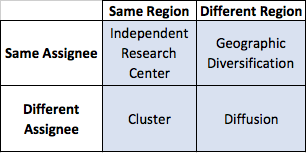
\includegraphics[width=0.8\textwidth]{2x2}
\end{centering}
\end{figure}

The top left quadrant, labelled an ``Independent Research Center" captures those knowledge flows that reflect competence building. Since these knowledge flows  are both within the region and within the firm, these flows represent local search on two dimensions (within firm and within region).  Thus, while the competence that is being built up by the Independent Research Center can be expected to have a positive effect on invention quality, the localness of the search on both dimensions may have a negative effect on invention quality. Figure~\ref{fig:SMSSameRegionSameAssigneeFlows} depicts the knowledge flows for this category (percentage of backward citations from this region that are to the same firm or assignee and same region) across time for five regions: Bangalore, Beijing, Tel Aviv-Yafo, Boston and San Jose (core of ``Silicon Valley"). While our empirical analysis covers all the major regions of the world, we chose these five regions as illustrative examples. We note that both San Jose and Boston report a higher proportion of knowledge flows within the same firm in the same region, while Bangalore and Tel Aviv-Yafo have the lowest proportion (fewer than 1\%) of their citations from the same firm within the same region. \par

\begin{figure}[h]
\begin{centering}
  \caption{Knowledge flows within regions and within assignees}
  \label{fig:SMSSameRegionSameAssigneeFlows}
  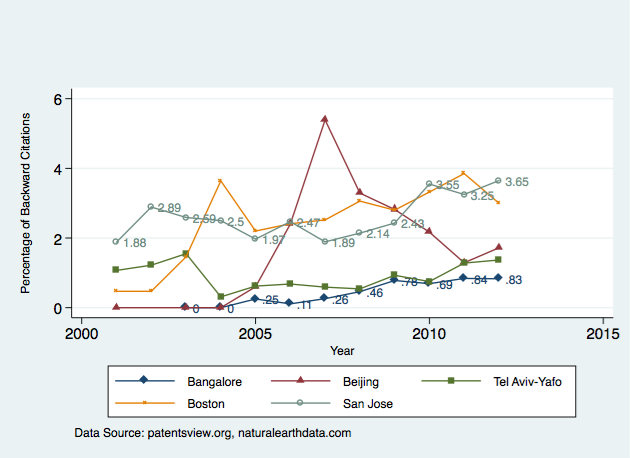
\includegraphics[width=0.90\textwidth]{SMSSameRegionSameAssigneeFlows}
\end{centering}
\end{figure}


The quadrant on the bottom left, labelled ``Cluster" captures knowledge spillovers within a region. Here firms may be seen as performing local search on one dimension (within regions) but not the other (within firms). Figure~\ref{fig:SMSSameRegionDiffAssigneeFlows} depicts the knowledge flows for this category across time for the same five regions. San Jose clearly stands out from the rest, suggesting a higher amount of across firm flows of knowledge in Silicon Valley, a result consistent with several prior studies. \par

\begin{figure}[h!]
\begin{centering}
  \caption{Knowledge flows within regions and across assignees}
  \label{fig:SMSSameRegionDiffAssigneeFlows}
  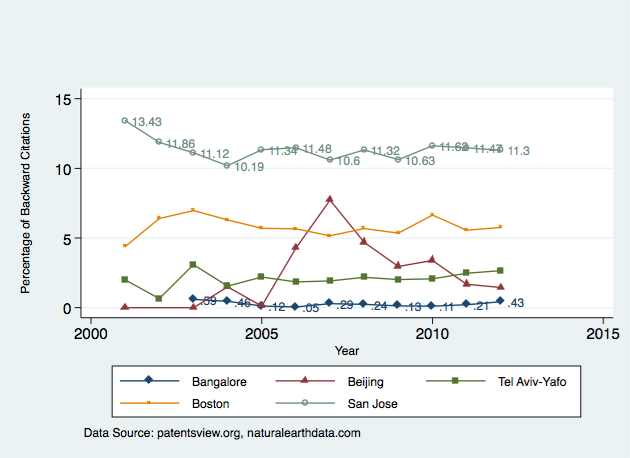
\includegraphics[width=0.90\textwidth]{SMSSameRegionDiffAssigneeFlows}
\end{centering}
\end{figure}

The quadrant on the top right, labelled as ``Geographic Diversification" captures local search on the dimension of the firm (across geographies) but not across regions. Innovations that are built on knowledge from several regions can be expected to benefit from the diversity of knowledge across regions. Yet, as in the previous quadrant, there is localness along the dimension of firm and such localness can have a negative effect on invention quality \citep{Rosenkopf2001}. Figure~\ref{fig:SMSDiffRegionSameAssigneeFlows} depicts the  knowledge flows for this category across time for the five regions. We note that Bangalore and Beijing have a relatively higher proportion of knowledge flows from same assignees in different locations, thus confirming the role of these regions as R\&D outposts of multinational firms.\par

\begin{figure}[h!]
\begin{centering}
  \caption{Knowledge flows across regions and within assignees}
  \label{fig:SMSDiffRegionSameAssigneeFlows}
  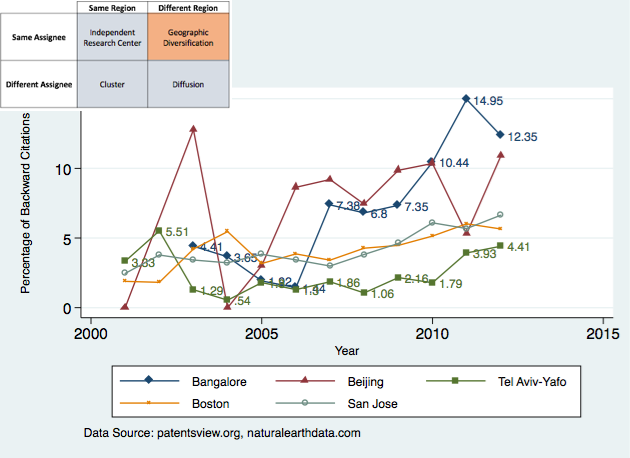
\includegraphics[width=0.90\textwidth]{SMSDiffRegionSameAssigneeFlows}
\end{centering}
\end{figure}

Finally, the bottom right quadrant labelled ``Diffusion" captures high exploration along both dimensions, indicating the development of a global pipeline \citep*{Bathelt2004}. Figure~\ref{fig:SMSDiffRegionDiffAssigneeFlows} depicts the  knowledge flows for this category across time for the five regions. We note that Bangalore, Beijing and Tel Avis-Yafo have a higher level of knowledge flows from other firms in other regions compared to Boston and San Jose, which is to be expected given that the absolute level of innovative activity in these emerging hotspots is still lower compared to that in Boston and San Jose. \par

\begin{figure}[h!]
\begin{centering}
  \caption{Knowledge flows across regions and across assignees}
  \label{fig:SMSDiffRegionDiffAssigneeFlows}
  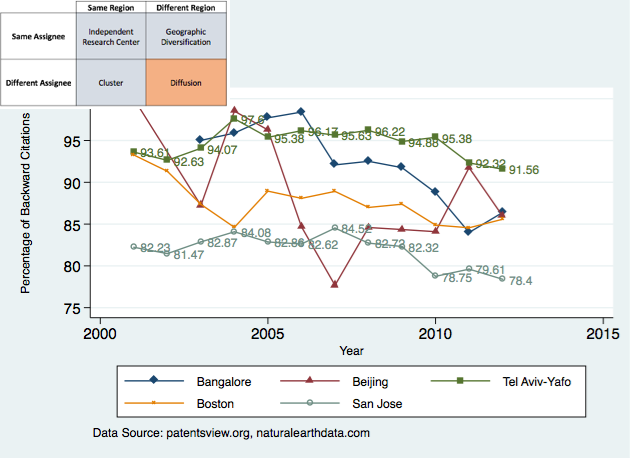
\includegraphics[width=0.90\textwidth]{SMSDiffRegionDiffAssigneeFlows}
\end{centering}
\end{figure}

As can be seen from the preceding discussion, prior theory suggests both positive and negative effects for each of these four categories of knowledge flows and it is not clear what the net effect will be on invention quality. This also suggests that prior theory does not provide guidance on which category of knowledge flows will have the highest effect on invention quality.  Since theory does not provide us with an answer, we rely on empirical analysis to inform us on the net effect of each category of knowledge flow on invention quality and which category has the highest effect on invention quality. \par


\subsubsection{Invention quality at the independent research center}
Organization learning literature suggests that specialized knowledge is routinized over time. As the dependence on FSHC reduces due to routinization of knowledge and the associated causal ambiguity arising out of tacit knowledge, the appropriability of rents by highly knowledgable workers reduces. Therefore managers intending to increase rents from exploration may chose a strategy where the rents from innovation are appropriated by highly skilled workers in the short run, but rents accrue to the firm as knowledge present in highly knowledgable workers is transformed into organizational routines. This leads me to my first hypothesis.\\

\begin{hypothesis}
{Hypothesis 1: Long term rent generating capacity of firms from exploration is characterized by an increase in costs due to appropriation by highly knowledgable employees initially, and a decrease in such costs later.
\\}
\end{hypothesis}

\subsubsection{Invention quality in a cluster}
 Contrary to Marshall?s findings, relating to urban specialization, \cite{Jacobs1969} points to the significance
of urban diversity as a source of external inputs that boost creativity and subsequently economic
activity. The main argument in this context is that the diversity found in agglomerations fosters
and enhances the cross-fertilization of ideas between industrial sectors. Although \cite{Marshall1890} already recognized the inherent risk that a strictly localized industry produces in terms of
vulnerability to external shocks in demand, or local labor uniformity that excludes certain segments of the
population from participating, it was Jacobs? account that stressed the importance of diversity to economic
development. In this context, development is considered growth through diversification, as the crossfertilization
of knowledge and technology between diverse sectors in the economy leads to the differentiation,
diversification, and transformation of the underlying processes of production, which in turn directly
influences total factor productivity (Ellerman, 2005). The results are mixed, and in some cases Marshall?Arrow?Romer (MAR)
externalities2 are considered more prevalent \citep{Baptista1998}, while in others, Jacobs?
externalities \citep{Feldman1999} are thought to dictate local knowledge spillover processes,
and in some instances both types of externalities are found to be significant \citep{Capello2002}. Marshallian externalities, which are concerned with intraindustry economies of localization, are
different from Jacobs? externalities that refer to interindustry exchanges between different technologies
and sectors within a particular metropolitan area, and therefore are not a mutually exclusive phenomenon
\citep*{Ibrahim2009}. The potential to generate radical, disruptive innovative output should be higher when very
diverse sectoral knowledge bases are combined, while incremental innovation should demand
specialized knowledge, which is necessary to improve existing technologies \citep{Schumpeter1942}.\\
 
\begin{hypothesis}
{Hypothesis 2: Given a certain organizational learning strategy for a firm, the short term profit performance in firms varies inversely with the extent of FSHC employed in the firm\\}
\end{hypothesis}

\subsubsection{Invention quality under geographical diversification}
IB literature has focused on issues such as the location
of R\&D \citep{Cantwell2000} and
the importance of agglomeration more generally
in explaining the location of internationally
mobile investments, . \cite{Nachum2000}, for example, offers a link between models
based on economic geography and IB analysis. \cite{Pantzalis2001} demonstrates that the location of foreign
subsidiaries can contribute significantly to the
value of the parent company, while \cite{Zaheer2001} address this issue of agglomeration
more explicitly. Expected benefits from
the location of a foreign affiliate in a business
cluster are associated with the presence of a
skilled labour market, a pool of specialized suppliers
and potential access to localized knowledge
assets. Potential threats are related to the presence
of a large pool of highly competitive firms specialized
in similar market segments or niches. This leads me to my first hypothesis.\\
\begin{hypothesis}
{Hypothesis 1: Long term rent generating capacity of firms from exploration is characterized by an increase in costs due to appropriation by highly knowledgable employees initially, and a decrease in such costs later.
\\}
\end{hypothesis}

\subsubsection{Invention quality under diffusion}
\cite{Breschi2005} argue that spatial
proximity is used by most localized knowledge
spillover studies as a proxy for social proximity.
To the extent that many social networks are concentrated
in space, spatial proximity would appear
as a significant determinant of access to knowledge
spillovers. If this is true, by replacing spatial
proximity with direct measurers of social proximity
we diminish the importance of geography as an
explanatory variable of spillovers. \cite{Breschi2009}, after controlling for patent inventors?
mobility and for the resulting co-invention
network, find that the residual effect of spatial
proximity on knowledge diffusion is greatly
reduced for invention.
 This leads me to my second hypothesis.\\

\begin{hypothesis}
{Hypothesis 2: Given a certain organizational learning strategy for a firm, the short term profit performance in firms varies inversely with the extent of FSHC employed in the firm\\}
\end{hypothesis}

\section*{Research Design}
Describe the two data sources, and the process taken. Assumptions made.

\begin{center}
\begin{table}[htbp]\centering \caption{Correlation Table for Dataset of Applicant \& Examiner Citations \label{ae.corrtable}}
\scriptsize
\singlespacing
\begin{adjustbox}{angle=0}
\begin{tabular}{l  c  c  c  c  c  c  c  c  c  c }

\hline
\multicolumn{1}{c}{Variables} &1&2&3&4&5&6&7&8&9&10\\ \hline
1. Total Citations Received&1.00\\
2. Non-Self Citations Received&0.98&1.00\\
3. Self Citations Received&0.88&0.78&1.00\\
4. Share Citations Made[Same Region, Same Assignee]&0.05&0.04&0.06&1.00\\
5. Share Citations Made[Same Region, Different Assignee]&0.11&0.11&0.09&0.04&1.00\\
6. Share Citations Made[Different Region, Same Assignee]&0.00&-0.01&0.03&0.20&-0.03&1.00\\
7. Share Citations Made[Different Region, Different Assignee]&0.05&0.05&0.03&-0.22&-0.05&-0.24&1.00\\
8. Log (Total Citations Made)&0.39&0.36&0.36&0.10&0.07&0.10&0.15&1.00\\
9. Log (Num Patents)&0.31&0.29&0.27&0.12&0.14&0.04&0.18&0.83&1.00\\
10. Log (Patent Pool Size)&0.27&0.25&0.24&0.17&0.14&0.06&0.06&0.76&0.86&1.00\\ \hline
\end{tabular}
\end{adjustbox}
\end{table}
\end{center}



\begin{table}[htbp]\centering \caption{Summary Statistics for Dataset of Applicant \& Examiner Citations\label{ae.sumstat}}
\scriptsize
\singlespacing
\begin{tabular}{l c c  c}\hline\hline
\multicolumn{1}{c}{\textbf{Variable}} & \textbf{Mean}
 & \textbf{Std. Dev.} & \textbf{N}\\ \hline
Total Citations Received & 241.719 & 2063.915  & 57456\\
Non-Self Citations Received& 123.856 & 1147.495  & 57456\\
Self Citations Received& 36.581 & 360.104  & 57456\\
Share Citations Made[Same Region, Same Assignee] & 0.042 & 0.087  & 24324\\
Share Citations Made[Same Region, Different Assignee] & 0.015 & 0.05  & 24324\\
Share Citations Made[Different Region, Same Assignee] & 0.069 & 0.119  & 24324\\
Share Citations Made[Different Region, Different Assignee] & 0.444 & 0.258  & 24324\\
Log (Total Citations Made) & 3.55 & 2.237  & 24324\\
Log (Num Patents) & 2.263 & 1.94  & 57456\\
Log (Patent Pool Size) & 4.59 & 2.373  & 54716\\
\hline
\end{tabular}
\end{table}

\begin{table}[htbp]\centering \caption{Regression Analysis of Invention Quality for Applicant \& Examiner Citations \label{ae.model123192021}}
\scriptsize
\singlespacing
\begin{tabular}{l*{6}{c}} \hline
                &\multicolumn{1}{c}{(1)}&\multicolumn{1}{c}{(2)}&\multicolumn{1}{c}{(3)}&\multicolumn{1}{c}{(4)}&\multicolumn{1}{c}{(5)}&\multicolumn{1}{c}{(6)}\\
                &\multicolumn{1}{c}{Total}&\multicolumn{1}{c}{Total}&\multicolumn{1}{c}{Total}&\multicolumn{1}{c}{Non-Self}&\multicolumn{1}{c}{Non-Self}&\multicolumn{1}{c}{Non-Self}\\
                &\multicolumn{1}{c}{Citations}&\multicolumn{1}{c}{Citations}&\multicolumn{1}{c}{Citations}&\multicolumn{1}{c}{Citations}&\multicolumn{1}{c}{Citations}&\multicolumn{1}{c}{Citations}\\
                 &\multicolumn{1}{c}{Received}&\multicolumn{1}{c}{Received}&\multicolumn{1}{c}{Received}&\multicolumn{1}{c}{Received}&\multicolumn{1}{c}{Received}&\multicolumn{1}{c}{Received}\\
\hline
Share Citations Made[Same Region, Same Assignee]&    0.211&    0.179&    0.254&    0.826&    0.899&    0.831\\
                &  (0.014)&  (0.128)&  (0.036)&  (0.000)&  (0.000)&  (0.000)\\
Share Citations Made[Same Region, Different Assignee]&   -0.393&   -0.471&  -0.0458&    0.816&    0.809&    0.811\\
                &  (0.010)&  (0.041)&  (0.808)&  (0.000)&  (0.003)&  (0.000)\\
Share Citations Made[Different Region, Same Assignee]&    0.244&    0.282&    0.326&    0.673&    0.655&    0.678\\
                &  (0.000)&  (0.002)&  (0.000)&  (0.000)&  (0.000)&  (0.000)\\
Share Citations Made[Different Region, Different Assignee]&  0.00301&   0.0243&    0.101&    0.820&    0.934&    0.802\\
                &  (0.932)&  (0.649)&  (0.036)&  (0.000)&  (0.000)&  (0.000)\\
Log (Total Citations Made)&    0.241&    0.193&    0.240&    0.180&    0.126&    0.214\\
                &  (0.000)&  (0.000)&  (0.000)&  (0.000)&  (0.000)&  (0.000)\\
Log (Num Patents)&    0.570&    0.662&    0.612&    0.634&    0.701&    0.620\\
                &  (0.000)&  (0.000)&  (0.000)&  (0.000)&  (0.000)&  (0.000)\\
Log (Patent Pool Size)&   -0.125&   -0.272&  -0.0931&  -0.0783&   -0.128&  -0.0734\\
                &  (0.000)&  (0.000)&  (0.000)&  (0.000)&  (0.000)&  (0.000)\\
Constant        &  -0.0147&    0.753&   -0.273&   -1.008&   -0.889&   -1.029\\
                &  (0.777)&  (0.000)&  (0.000)&  (0.000)&  (0.000)&  (0.000)\\
\hline
Observations    &    16111&     6449&     9662&    15701&     6324&     9377\\
Groups          &     1776&      617&     1159&     1654&      587&     1067\\
Sample&All &U.S. &Non-U.S.&All &U.S. &Non-U.S. \\
          &Locations &Locations&Locations&Locations &Locations&Locations \\
\hline\hline
\multicolumn{7}{l}{\footnotesize \textit{p}-values in parentheses}\\
\multicolumn{7}{l}{\footnotesize All regressions use negative binomial estimation on the region-year panel}\\
\multicolumn{7}{l}{\footnotesize Citations received are counted up to and including the fifth annual anniversary of a patent application}\\
\multicolumn{7}{l}{\footnotesize All models include region fixed effects, year dummies and technology subcategory controls}\\
\end{tabular}
\end{table}


\normalsize
\onehalfspacing

\section*{Data and Methods}

We use patent citations data from the U.S. Patent Office (USPTO) as provided by patentsview.org. The USPTO provides information on assignee, the location of inventors, and year of patent application. We use this information to identify which patents belong to which region in a given year. Since there can be more than one inventor on a patent, a patent can belong to more than one region. We compare the assignee and inventor location of each patent with each assignee and inventor of each backward citation  to identify the category of knowledge flow (e.g., same assignee, different location) indicated by the backward citation. Additionally, to map location data of inventors from USPTO to regions, we use urban centers data for worldwide locations from \href{http://www.naturalearthdata.com/downloads/10m-cultural-vectors/}{Natural Earth Data} that uses remote sensing data to determine urban agglomerations (a process developed in \citet*{Schneider2003}).  While it has been common practice to use Metropolitan Statistical Areas (MSA) for analyses related to economic geography in the U.S., an equivalent measure is unavailable for the rest of the world. For comparability and consistency, we choose to use the urban centers definitions from \href{http://www.naturalearthdata.com/downloads/10m-cultural-vectors/}{Natural Earth Data} for all regions both within U.S. and outside U.S. \par
Our unit of analysis is the region-year. To be consistent with our objective of measuring knowledge flows, we restrict ourselves to those citations categorized as \textquotesingle cited by applicant\textquotesingle \ and leave out those categorized as \textquotesingle cited by examiner\textquotesingle \ because the latter may not represent knowledge flows. This decision has the additional effect of limiting our period of analysis to citing patents applied for after the year 2000 since the data on which citations were added by examiners is available for patents from only 2001 onwards. We restrict our sample to patents applied for between 2001 - 2012, but citations received till 2015. In models where citations are counted until the fifth annual anniversary, patent applications from 2011 and 2012 may be seen as being at a relative disadvantage. However, this must be corrected on updating the dataset to the version updated to March 2017. For paucity of time, the dataset was not updated in time for the submission of this paper.\par
\subsection{Dependent Variable}
Our primary dependent variable is the  total count of citations (received up to and including the fifth anniversary of the patent filing or until  2015, whichever is earlier) by patents belonging to a region-year. For robustness, we also report results for total non-self citations received as the dependent variable. 

\subsection{Independent Variables}
Our independent variables are the percentage of backward citations made to each of the four categories in our defined framework: those to a) same region, same assignee, b) same region, different assignee, c) different region, same assignee, and d) different region, same assignee. \par
\subsubsection{Percentage of backward citations made to same region and same assignee}
Write some text here. Include some mathematics here.
\subsubsection{Percentage of backward citations made to same region and different assignee}
Write some text here
\subsubsection{Percentage of backward citations made to different region and same assignee}
Write some text here
\subsubsection{Percentage of backward citations made to different region and different assignee}
Write some text here

\subsection{Control Variables}
We control for the total number of citations made in the region-year, the total number of patents in the region-year, the size of the patent pool in the region-year, as well as the percentage of patents in region-year in each technology subcategory as defined by \cite*{Hall2001a}. The patent pool is the total number of patents that belong to a region up to the previous year. It is important to control for the size of the patent pool as  regions that have a larger patent pool (such as San Jose) will have more patents that can be cited and can therefore have larger within region spillovers as compared to a region that has only a small patent pool. We include region fixed effects and year dummies in all regression models so as to control for region level and year specific effects, if any. Since our dependent variable is a count variable, we used negative binomial regression analysis with fixed effects. \par

\section*{Model Estimation}
Some text followed by mathematical formula estimated

\section*{Results}
The preliminary results from our analysis are presented in Table~\ref{model123}. Model 1 reports the results for all regions worldwide, while Model 2 and Model 3 report results for U.S. locations and non-U.S. locations respectively. Across the three models we find that local knowledge flows within the firm do not seem to have a significant impact on the quality of inventions as measured by the number of citations received. This result is robust to using non-self citations as the dependent variable as presented in Table~\ref{model192021}. \par
Our preliminary findings in Table~\ref{model123} suggest no evidence that local knowledge spillovers (i.e., same region, different assignee) lead to higher quality inventions.  One possible explanation for the lack of evidence for local knowledge spillovers may be to suggest U.S. specific effects. However as the results in model 2 of Table~\ref{model123} suggest, the trend is confirmed in a U.S.-only sample. It seems therefore that the implication for the lack of effect of localized knowledge flows on invention quality is robust to regional or country sampling. \par
The effect of non-local knowledge flows however is less clear. While geographic diversification is seen to benefit all regions (Table~\ref{model123}), the effect is not statistically significant for non-U.S. locations (Table~\ref{model192021}). This may suggest that there are regional, and potentially country effects that may be able to explain the phenomenon better. Finally, building on knowledge from outside the firm and outside the region does not seem to improve invention quality.\par

\subsection{Robustness Checks}





\begin{center}
\begin{table}[htbp]\centering \caption{Correlation Table for Dataset of Examiner Citations Only \label{e.corrtable}}
\scriptsize
\singlespacing
\begin{adjustbox}{angle=0}
\begin{tabular}{l  c  c  c  c  c  c  c  c  c  c }

\hline
\multicolumn{1}{c}{Variables} &1&2&3&4&5&6&7&8&9&10\\ \hline
1. Total Citations Received&1.00\\
2. Non-Self Citations Received&0.99&1.00\\
3. Self Citations Received&0.91&0.88&1.00\\
4. Share Citations Made[Same Region, Same Assignee]&0.04&0.03&0.06&1.00\\
5. Share Citations Made[Same Region, Different Assignee]&0.11&0.11&0.11&0.03&1.00\\
6. Share Citations Made[Different Region, Same Assignee]&-0.00&-0.01&0.02&0.23&-0.03&1.00\\
7. Share Citations Made[Different Region, Different Assignee]&0.05&0.05&0.04&-0.22&-0.05&-0.22&1.00\\
8. Log (Total Citations Made)&0.37&0.34&0.40&0.09&0.07&0.08&0.17&1.00\\
9. Log (Num Patents)&0.29&0.27&0.30&0.12&0.14&0.05&0.17&0.84&1.00\\
10. Log (Patent Pool Size)&0.25&0.23&0.26&0.17&0.13&0.05&0.06&0.75&0.86&1.00\\ \hline
\end{tabular}
\end{adjustbox}
\end{table}
\end{center}



\begin{table}[htbp]\centering \caption{Summary Statistics for Dataset of Examiner Citations Only \label{e.sumstat}}
\scriptsize
\singlespacing
\begin{tabular}{l c c  c}\hline\hline
\multicolumn{1}{c}{\textbf{Variable}} & \textbf{Mean}
 & \textbf{Std. Dev.} & \textbf{N}\\ \hline
Total Citations Received & 169.117 & 1518.954  & 57456\\
Non-Self Citations Received& 91.528 & 916.089  & 57456\\
Self Citations Received& 21.64 & 188.776  & 57456\\
Share Citations Made[Same Region, Same Assignee] & 0.042 & 0.086  & 23757\\
Share Citations Made[Same Region, Different Assignee] & 0.014 & 0.049  & 23757\\
Share Citations Made[Different Region, Same Assignee] & 0.061 & 0.111  & 23757\\
Share Citations Made[Different Region, Different Assignee] & 0.447 & 0.261  & 23757\\
Log (Total Citations Made) & 3.378 & 2.147  & 23757\\
Log (Num Patents) & 2.263 & 1.94  & 57456\\
Log (Patent Pool Size) & 4.59 & 2.373  & 54716\\
\hline
\end{tabular}
\end{table}

\begin{table}[htbp]\centering \caption{Regression Analysis of Invention Quality for Examiner Citations Only \label{e.model123192021}}
\scriptsize
\singlespacing
\begin{tabular}{l*{6}{c}} \hline
                &\multicolumn{1}{c}{(1)}&\multicolumn{1}{c}{(2)}&\multicolumn{1}{c}{(3)}&\multicolumn{1}{c}{(4)}&\multicolumn{1}{c}{(5)}&\multicolumn{1}{c}{(6)}\\
                &\multicolumn{1}{c}{Total}&\multicolumn{1}{c}{Total}&\multicolumn{1}{c}{Total}&\multicolumn{1}{c}{Non-Self}&\multicolumn{1}{c}{Non-Self}&\multicolumn{1}{c}{Non-Self}\\
                &\multicolumn{1}{c}{Citations}&\multicolumn{1}{c}{Citations}&\multicolumn{1}{c}{Citations}&\multicolumn{1}{c}{Citations}&\multicolumn{1}{c}{Citations}&\multicolumn{1}{c}{Citations}\\
                 &\multicolumn{1}{c}{Received}&\multicolumn{1}{c}{Received}&\multicolumn{1}{c}{Received}&\multicolumn{1}{c}{Received}&\multicolumn{1}{c}{Received}&\multicolumn{1}{c}{Received}\\
\hline
Share Citations Made[Same Region, Same Assignee]&    0.289&    0.151&    0.437&    0.929&    0.981&    0.925\\
                &  (0.000)&  (0.168)&  (0.000)&  (0.000)&  (0.000)&  (0.000)\\
Share Citations Made[Same Region, Different Assignee]&    0.279&  -0.0690&    0.510&    1.278&    0.765&    1.358\\
                &  (0.059)&  (0.756)&  (0.009)&  (0.000)&  (0.009)&  (0.000)\\
Share Citations Made[Different Region, Same Assignee]&    0.169&   0.0516&    0.270&    0.662&    0.446&    0.777\\
                &  (0.007)&  (0.571)&  (0.002)&  (0.000)&  (0.000)&  (0.000)\\
Share Citations Made[Different Region, Different Assignee]&   0.0489&   0.0463&    0.135&    0.961&    1.100&    0.907\\
                &  (0.156)&  (0.346)&  (0.005)&  (0.000)&  (0.000)&  (0.000)\\
Log (Total Citations Made)&    0.377&    0.331&    0.395&    0.410&    0.367&    0.430\\
                &  (0.000)&  (0.000)&  (0.000)&  (0.000)&  (0.000)&  (0.000)\\
Log (Num Patents)&    0.479&    0.552&    0.500&    0.433&    0.483&    0.448\\
                &  (0.000)&  (0.000)&  (0.000)&  (0.000)&  (0.000)&  (0.000)\\
Log (Patent Pool Size)&   -0.112&   -0.236&   -0.113&  -0.0856&   -0.141&  -0.0999\\
                &  (0.000)&  (0.000)&  (0.000)&  (0.000)&  (0.000)&  (0.000)\\
Constant        &    0.409&    1.230&    0.169&   -0.688&   -0.441&   -0.688\\
                &  (0.000)&  (0.000)&  (0.010)&  (0.000)&  (0.001)&  (0.000)\\
\hline
Observations    &    15760&     6362&     9398&    15345&     6225&     9120\\
Groups          &     1738&      611&     1127&     1619&      581&     1038\\
Sample&All &U.S. &Non-U.S.&All &U.S. &Non-U.S. \\
          &Locations &Locations&Locations&Locations &Locations&Locations \\
\hline\hline
\multicolumn{7}{l}{\footnotesize \textit{p}-values in parentheses}\\
\multicolumn{7}{l}{\footnotesize All regressions use negative binomial estimation on the region-year panel}\\
\multicolumn{7}{l}{\footnotesize Citations received are counted up to and including the fifth annual anniversary of a patent application}\\
\multicolumn{7}{l}{\footnotesize All models include region fixed effects, year dummies and technology subcategory controls}\\
\end{tabular}
\end{table}



\begin{center}
\begin{table}[htbp]\centering \caption{Correlation Table for Dataset of Applicant Citations Only \label{a.corrtable}}
\scriptsize
\singlespacing
\begin{adjustbox}{angle=0}
\begin{tabular}{l  c  c  c  c  c  c  c  c  c  c }

\hline
\multicolumn{1}{c}{Variables} &1&2&3&4&5&6&7&8&9&10\\ \hline
1. Total Citations Received&1.00\\
2. Non-Self Citations Received&0.95&1.00\\
3. Self Citations Received&0.93&0.78&1.00\\
4. Share Citations Made[Same Region, Same Assignee]&0.03&0.02&0.04&1.00\\
5. Share Citations Made[Same Region, Different Assignee]&0.08&0.09&0.06&0.01&1.00\\
6. Share Citations Made[Different Region, Same Assignee]&-0.01&-0.03&0.01&0.12&-0.07&1.00\\
7. Share Citations Made[Different Region, Different Assignee]&0.05&0.06&0.02&-0.29&-0.07&-0.35&1.00\\
8. Log (Total Citations Made)&0.38&0.37&0.33&0.07&0.08&0.10&0.05&1.00\\
9. Log (Num Patents)&0.24&0.25&0.18&0.05&0.11&-0.02&0.18&0.72&1.00\\
10. Log (Patent Pool Size)&0.21&0.22&0.16&0.11&0.11&-0.01&0.05&0.69&0.86&1.00\\ \hline
\end{tabular}
\end{adjustbox}
\end{table}
\end{center}



\begin{table}[htbp]\centering \caption{Summary Statistics for Dataset of Applicant Citations Only \label{a.sumstat}}
\scriptsize
\singlespacing
\begin{tabular}{l c c  c}\hline\hline
\multicolumn{1}{c}{\textbf{Variable}} & \textbf{Mean}
 & \textbf{Std. Dev.} & \textbf{N}\\ \hline
Total Citations Received & 72.602 & 818.182  & 57456\\
Non-Self Citations Received& 32.328 & 348.87  & 57456\\
Self Citations Received& 14.942 & 227.598  & 57456\\
Share Citations Made[Same Region, Same Assignee] & 0.056 & 0.114  & 10243\\
Share Citations Made[Same Region, Different Assignee] & 0.021 & 0.064  & 10243\\
Share Citations Made[Different Region, Same Assignee] & 0.109 & 0.165  & 10243\\
Share Citations Made[Different Region, Different Assignee] & 0.431 & 0.28  & 10243\\
Log (Total Citations Made) & 3.374 & 2.186  & 10243\\
Log (Num Patents) & 2.263 & 1.94  & 57456\\
Log (Patent Pool Size) & 4.59 & 2.373  & 54716\\\hline
\end{tabular}
\end{table}

\begin{table}[htbp]\centering \caption{Regression Analysis of Invention Quality for Applicant Citations Only \label{a.model123192021}}
\scriptsize
\singlespacing
\begin{tabular}{l*{6}{c}} \hline
                &\multicolumn{1}{c}{(1)}&\multicolumn{1}{c}{(2)}&\multicolumn{1}{c}{(3)}&\multicolumn{1}{c}{(4)}&\multicolumn{1}{c}{(5)}&\multicolumn{1}{c}{(6)}\\
                &\multicolumn{1}{c}{Total}&\multicolumn{1}{c}{Total}&\multicolumn{1}{c}{Total}&\multicolumn{1}{c}{Non-Self}&\multicolumn{1}{c}{Non-Self}&\multicolumn{1}{c}{Non-Self}\\
                &\multicolumn{1}{c}{Citations}&\multicolumn{1}{c}{Citations}&\multicolumn{1}{c}{Citations}&\multicolumn{1}{c}{Citations}&\multicolumn{1}{c}{Citations}&\multicolumn{1}{c}{Citations}\\
                 &\multicolumn{1}{c}{Received}&\multicolumn{1}{c}{Received}&\multicolumn{1}{c}{Received}&\multicolumn{1}{c}{Received}&\multicolumn{1}{c}{Received}&\multicolumn{1}{c}{Received}\\
\hline
Share Citations Made[Same Region, Same Assignee]&   -0.125&   -0.150&  -0.0872&   -0.256&   -0.302&   -0.240\\
                &  (0.184)&  (0.290)&  (0.490)&  (0.017)&  (0.065)&  (0.100)\\
Share Citations Made[Same Region, Different Assignee]&   -0.229&   -0.281&  -0.0944&    0.252&    0.222&    0.253\\
                &  (0.116)&  (0.245)&  (0.599)&  (0.097)&  (0.393)&  (0.187)\\
Share Citations Made[Different Region, Same Assignee]&    0.114&    0.217&   0.0820&   0.0375&    0.109&  -0.0360\\
                &  (0.080)&  (0.023)&  (0.364)&  (0.622)&  (0.326)&  (0.733)\\
Share Citations Made[Different Region, Different Assignee]&  -0.0703&  -0.0400&  -0.0725&  -0.0220&   0.0199&  -0.0546\\
                &  (0.107)&  (0.535)&  (0.221)&  (0.647)&  (0.782)&  (0.405)\\
Log (Total Citations Made)&   0.0556&   0.0464&   0.0596&   0.0378&   0.0210&   0.0423\\
                &  (0.000)&  (0.000)&  (0.000)&  (0.000)&  (0.030)&  (0.000)\\
Log (Num Patents)&    0.712&    0.780&    0.700&    0.720&    0.768&    0.743\\
                &  (0.000)&  (0.000)&  (0.000)&  (0.000)&  (0.000)&  (0.000)\\
Log (Patent Pool Size)&  -0.0436&   -0.153&  0.00211&   0.0188&  -0.0287&-0.0000276\\
                &  (0.075)&  (0.000)&  (0.950)&  (0.509)&  (0.542)&  (0.999)\\
Constant        &   -2.621&   -2.141&   -2.944&   -3.255&   -2.997&   -3.380\\
                &  (0.000)&  (0.000)&  (0.000)&  (0.000)&  (0.000)&  (0.000)\\
\hline
Observations    &     7275&     3434&     3841&     7080&     3357&     3723\\
Groups          &     1095&      483&      612&     1019&      454&      565\\
Sample&All &U.S. &Non-U.S.&All &U.S. &Non-U.S. \\
          &Locations &Locations&Locations&Locations &Locations&Locations \\
\hline\hline
\multicolumn{7}{l}{\footnotesize \textit{p}-values in parentheses}\\
\multicolumn{7}{l}{\footnotesize All regressions use negative binomial estimation on the region-year panel}\\
\multicolumn{7}{l}{\footnotesize Citations received are counted up to and including the fifth annual anniversary of a patent application}\\
\multicolumn{7}{l}{\footnotesize All models include region fixed effects, year dummies and technology subcategory controls}\\
\end{tabular}
\end{table}

\begin{table}[htbp]\centering \caption{Regression Analysis of Invention Quality* for Applicant Citations Only \label{ainf.model123192021}}
\scriptsize
\singlespacing
\begin{tabular}{l*{6}{c}} \hline
                &\multicolumn{1}{c}{(1)}&\multicolumn{1}{c}{(2)}&\multicolumn{1}{c}{(3)}&\multicolumn{1}{c}{(4)}&\multicolumn{1}{c}{(5)}&\multicolumn{1}{c}{(6)}\\
                &\multicolumn{1}{c}{Total}&\multicolumn{1}{c}{Total}&\multicolumn{1}{c}{Total}&\multicolumn{1}{c}{Non-Self}&\multicolumn{1}{c}{Non-Self}&\multicolumn{1}{c}{Non-Self}\\
                &\multicolumn{1}{c}{Citations}&\multicolumn{1}{c}{Citations}&\multicolumn{1}{c}{Citations}&\multicolumn{1}{c}{Citations}&\multicolumn{1}{c}{Citations}&\multicolumn{1}{c}{Citations}\\
                 &\multicolumn{1}{c}{Received}&\multicolumn{1}{c}{Received}&\multicolumn{1}{c}{Received}&\multicolumn{1}{c}{Received}&\multicolumn{1}{c}{Received}&\multicolumn{1}{c}{Received}\\
\hline
Share Citations Made[Same Region, Same Assignee]&   -0.169         &   -0.104         &   -0.134&-0.232         &   -0.183         &   -0.316 \\
                &   (0.218)         &  (0.623)         &  (0.454)&   (0.105)         &  (0.392)         &  (0.123) \\
Share Citations Made[Same Region, Different Assignee]&    -0.149         &   -0.191         &  -0.0919&    0.0391         &   0.0945         &   0.0505 \\
                &   (0.215)         &  (0.458)         &  (0.468) &   (0.733)         &  (0.721)         &  (0.699) \\
Share Citations Made[Different Region, Same Assignee]&     0.217  &    0.266  &    0.348&    0.195  &    0.263  &    0.174 \\
                &(0.012)         &  (0.037)         &  (0.004) &   (0.035)         &  (0.041)         &  (0.212)\\
Share Citations Made[Different Region, Different Assignee]&  0.00828         &   0.0315         &   0.0179&   0.00989         &   0.0203         &  0.00983  \\
                &  (0.789)         &  (0.499)         &  (0.661)&    (0.762)         &  (0.675)         &  (0.826)         \\
Log (Total Citations Made)&    0.0180&   0.0198&   0.0134&     0.0150&   0.0139  &   0.0107 \\
                &   (0.000)         &  (0.001)         &  (0.014)&   (0.000)         &  (0.023)         &  (0.075) \\
Log (Num Patents)&     0.785&    0.811&    0.830&        0.772&    0.795&    0.828\\
                &  (0.000)         &  (0.000)         &  (0.000)&  (0.000)&  (0.000)&  (0.000)\\
Log (Patent Pool Size)&  -0.111&   -0.227&  -0.0944&    -0.0453  &   -0.108 &  -0.0685\\
                &  (0.075)&  (0.000)&  (0.950)&   (0.039)         &  (0.006)         &  (0.017) \\
\hline
Observations    &    9241&3885&5356&          8879         &     3732         &     5147\\
Groups          &     1314&529&785&1199         &      478         &      721\\
Sample&All &U.S. &Non-U.S.&All &U.S. &Non-U.S. \\
          &Locations &Locations&Locations&Locations &Locations&Locations \\
\hline\hline
\multicolumn{7}{l}{\footnotesize \textit{p}-values in parentheses}\\
\multicolumn{7}{l}{\footnotesize All regressions use negative binomial estimation on the region-year panel}\\
\multicolumn{7}{l}{\footnotesize * Citations received are counted all the way to end 2016 for which data is available}\\
\multicolumn{7}{l}{\footnotesize All models include region fixed effects, year dummies and technology subcategory controls}\\
\end{tabular}
\end{table}


\section*{Discussion}
Lookup other articles to determine what points need to be made here.
\subsection{On topic 1}
\cite*{Henderson2005} provide comments on the reassessment of the JTH methodology carried out
by \cite{Thompson2005}, in particular they point to the possibility that the lack of localization
effects in the results, at the intranational scale, are due to a possible sample selection bias induced in
the final step of the TFK test, where the sample is restricted to control patents whose primary subclass
matches the primary subclass of the citing patent. The key problem, identified by Henderson et al.
(2005), with the methodology applied in the TFK experiment relates to the missing justification as to
why spillovers should only occur within the narrowly defined subclasses. An analysis that relies
fundamentally on intratechnology flows would follow the argument of specialization, but at the same
time would certainly exclude any possible evidence pertaining to knowledge spillovers from other
technology sectors in the process of invention, thus rendering arguments for diversification inadequate.
 Controlling for the geographic and temporal distribution
of ?technology in order to identify knowledge spillovers is very tricky, and [. . .] the exercise in JTH can
hardly be regarded as conclusive in that respect? \citep*{Henderson2005}. This suggests that
further research is warranted.
\cite{Maurseth2002} offer an alternative approach for capturing technological linkages,
which has been an area of criticism in the JTH methodology, by constructing a regional compatibility
index for all regions across Europe; however, they derived similar results, which also indicate that
geography matters. Furthermore, studies that examine whether or not the strong proximity effect of
knowledge spillovers found in macrolevel studies also holds true in a microcontext, generally confirm
the proximity effect on spillovers, and find significant negative coefficients on the geographical and
technological distance variables \citep{Verspagen2004}.
Patent citation analysis is not the only research framework that may be utilized to quantify knowledge
externalities. An alternative stream of analysis focuses on the movement of people, and is based upon
the idea that knowledge is embedded within an individual. In contrast to patent citation analysis, which
focused on the mapping of codified knowledge, research undertaken in this context attempts to measure
the flow of tacit knowledge \cite{Polanyi1958}, which is an equal pervasive but different part of knowledge

\subsection{On topic 2}
Geography provides
a platform to organize these interactions, and focusing on only one spatial scale will perhaps not be
sufficient to fully understand innovation processes \citep{Bunnell2001}. There are many distinctive
parts that shape economic activity in a particular place (Feldman and Martin, 2005). This includes notfor-
profit organizations, such as universities, research consortia, and standards setting organizations that
play a significant role in affecting scientific opportunity and the diffusion of innovation, or other public
entities, such as foundations that may fund research and help create markets.


Alternative explanations
\cite{Almeida1997} show that mobility patterns of star patent holders in the semiconductor
industry match the transfer of knowledge, and therefore directly influence the geographic patterns of
knowledge spillovers.\cite{Song2003} illustrate that mobile engineers who join a firm with stronger path
dependence are less likely to build upon the knowledge of their previous firms, especially if the
engineer?s key area of expertise lies inside the core technology areas of the new firm.

\section*{Limitations}
While the use of patent citations as a measure of knowledge flows has been popular in the literature, this may nevertheless be subject to error \citep*{Arora2017a}. Our definition of regions is dependent on the latitude/longitude assignment in the patentsview.org data and on the urban centers definition in the \href{http://www.naturalearthdata.com/downloads/10m-cultural-vectors/}{Natural Earth Data}. Any systematic biases in the definition of regions can create biases in measures of within region and across region knowledge flows. \par

\section*{Conclusion}
While still at a preliminary stage, our analysis seem to suggest that local knowledge flows as measured by patent citations may not have a significant effect on the quality of inventions produced in a region. This casts a doubt on the widely accepted idea that local knowledge spillovers are an important source of agglomeration economies. A potential extension of the study could be to conduct empirical analysis at the level of firm-year rather than at the region-year. We could additionally look at the additional dimension of technology (within and outside technological domain, \cite{Rosenkopf2001}) in addition to those of within/outside region and within/outside firm. This may provide us with a more nuanced understanding of the factors affecting invention quality. Future studies could potentially examine other measures of invention outcomes such as breakthrough inventions. Finally, while our work suggests that local knowledge spillovers do not affect invention quality, it is not quite as clear why this may be the case. We hope that our current work spurs further research in this direction.  

%\onehalfspacing
%\singlespacing
\renewcommand{\refname}{REFERENCES}
\singlespacing
\bibliography{/Users/aiyenggar/code/bibliography/aiyenggar} 
\bibliographystyle{ai-amjlike}
\newpage
%\normalsize

\end{document}
